\shorthandoff{"}
\chapter{Methodik}
\label{ch:methodik}

Zu erhebende Daten:\\
- Skills sind im Intranet gespeichert: Bewertung auf einer Skala von 1 bis 5\\
- Zusätzlich Teamzuordnung im Intranet --> Kantengewicht: 1\\
- Für jeden Mitarbeiter erheben: Wichtigkeit (true/false)\\
- Für jeden Mitarbeiter erheben: Welche Auswirkung hat es, wenn im Projekt nicht ausgelastet (Kurve A bis C)

Erstellen des Graphen:\\
- Aus Skills (kollaboratives Filtern) und Teamzuordnung (Inhaltsbasiertes Filtern) einen tripartiten Graphen erstellen\\
- Sinnvolle Kanten: Nutzer-Skill / Nutzer-Team // Besser: Nutzer-Skill und Nutzer-Manager --> Weniger Knoten\\
- Entscheidung gegen Mittelwertzentrierung

% Johannes: 404
% Jan: 366
% Alexander: 20
\begin{figure}[h]
	\centering	
	\begin{tikzpicture}[node distance={32mm}, thick, main/.style = {draw, circle}] 
		\node[main, fill=itemcolor] (MongoDB) {$MongoDB$}; 
		\node[main, fill=itemcolor] (Python) [below right of=MongoDB] {$Python$}; 
		\node[main, fill=itemcolor] (MySQL) [above right of=Python] {$MySQL$}; 
		\node[main, fill=itemcolor] (Java) [below right of=MySQL] {$Java$}; 
		\node[main, fill=itemcolor] (HDFS) [above right of=Java] {$HDFS$}; 
		\node[main, fill=itemcolor] (Spark) [below right of=HDFS] {$Spark$};
		
		\node[main, fill=usercolor] (Johannes) [above right of=MongoDB] {$Joh L.$}; 
		\node[main, fill=usercolor] (Jan) [above left of=HDFS] {$Jan H.$}; 
		\node[main, fill=usercolor] (Alexander) [above right of=HDFS] {$Alex G.$};
		
		\node[main, fill=exxetagray] (JES32) [above right of=Johannes] {$JES 3.2$};
		
		\draw (Johannes) -- node[midway, right] {4} (Python);
		\draw (Johannes) -- node[midway, above] {3} (MySQL);
		\draw (Johannes) -- node[midway, above] {3} (MongoDB);
		
		\draw (Jan) -- node[midway, right] {1} (HDFS);		
		\draw (Jan) -- node[midway, right] {3} (Java);
		\draw (Jan) -- node[midway, above] {2} (MySQL);
		
		\draw (Alexander) -- node[midway, above] {5} (HDFS);
		\draw (Alexander) -- node[midway, left] {3} (Spark);
		
		\draw (Johannes) -- node[midway, above] {1} (JES32);
		%\draw (Johannes) -- node[midway, above] {1} (Jan);
		\draw (Jan) -- node[midway, above] {1} (JES32);
	\end{tikzpicture}
	
	\caption{Darstellung der Fähigkeitsmatrix aus Tabelle \ref{tbl:empfehlungssysteme:arbeitsweise:tbl1} in der Datenstruktur eines Graphen}
	\label{fig:methodik:abb1}
\end{figure}

Eingabe der offenen Projektposition:\\
- Benötigt: Fähigkeiten und Wichtigkeit (Boolean)

Algorithmus:\\
- Berechnung der Katz-Zentralität\\
- Für jeden relevanten Mitarbeiter auf Basis von Abbildung \ref{fig:methodik:abb2} den finalen Wert bestimmen --> Hierbei je nach Wichtigkeit die Kurve stauchen --> Wenn für Projektmanger wichtig, die durchgezogene Linie doppelt so steil; Wenn für Mitarbeiter wichtig, rechte Seite doppelt so steil; Auswahl der Kurve anhand der Information des Mitarbeiters\\
- Summe für alle Fähigkeiten eines Projektes für jeden Mitarbeiter berechnen

\begin{figure}[h]
	\centering
	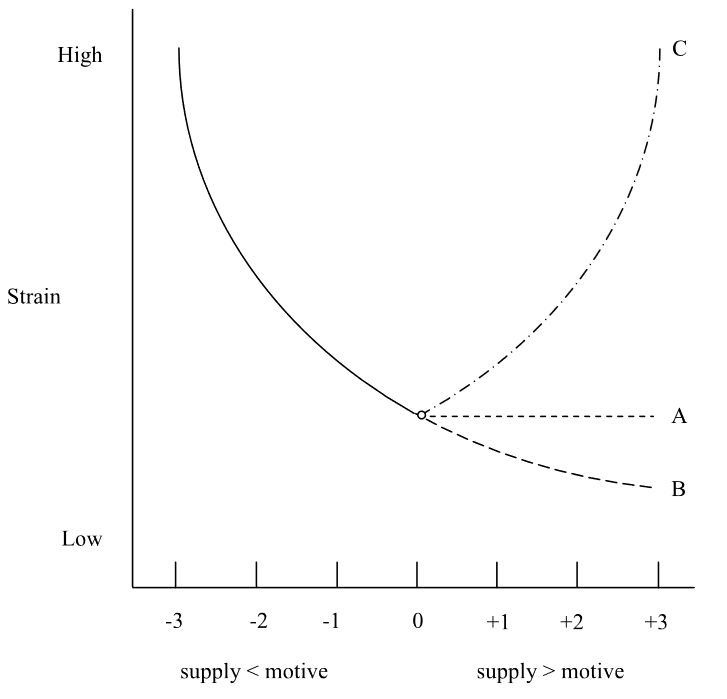
\includegraphics[width=0.75\textwidth]{gfx/ueberschuss_supply_motive.png}
	\caption{Auswirkungen eines Bedürfnisse-Angebote Misfits \cite[S. 23]{edwards:2008}\\(Bearbeitet von \myName)}
	\label{fig:methodik:abb2}
\end{figure}

- Algorithmus einmal durchführen mit Wichtigkeiten und einmal ohne (bilateral vs. unilateral)\\
- Ausgabe der sortierten Liste (mit allen Mitarbeitern (zB 25))\\
- Eingabe der Projektposition und Algorithmus für jede Projektposition wiederholen

Evaluation für Projektmanager:\\
- Erhält für jedes Projekt beide Listen und gibt auf einer Skala von 1 bis 5 an, wie hoch der die Leistung der empfohlenen Mitarbeiter in diesem Projekt einschätzen würde

Evaluation für Mitarbeiter:\\
- Jeder Mitarbeiter muss für jedes Projekt auf einer Skala von 1 bis 5 bewerten, wie zufrieden er wäre, wenn er darin arbeiten würde\\
- Ergebnisliste wird in Intervalle geteilt --> z.B. Zufriedenheit 5 bedeutet bei 25 Teilnehmern, dass der Nutzer im ersten Intervall sein muss --> Abweichung bestimmen --> Je weniger Abweichung, desto besser --> Durchschnittliche Abweichung von unilateral und bilateral vergleichen

Frage:\\
- Muss Manager überhaupt Wichtigkeiten angeben?
\shorthandon{"}
